\documentclass[12pt, letterpaper]{article}
\usepackage[left=1in, right=1in, top=1in, bottom=1in]{geometry}
\usepackage{subfiles}
\usepackage{C:/users/fores/format}
\title{\textbf{Notes on Convex Analysis and Nonlinear Optimization
by Borwein and Lewis}}
\author{Forest Yang }
\date{May 30 2019}
\numberwithin{equation}{subsection}
\begin{document}
\maketitle
\section{Chapter 1: Background}
\subsection{Euclidean spaces, basic definitions}
Consider a finite dimensional vector space equipped with inner product 
$\ip{\cdot,\cdot}$ and norm defined by $\|x\|=\sqrt{\ip{x,x}}$.
\begin{itemize}
\item $B:= \{x\in\R^n : \|x\|\leq 1\}$.
\item Sums, differences, and products of their sets are defined by 
doing the operation on all pairs of elements s.t. one is from each set.
\item Cone: a nonempty set $C$ such that $\R_+C=C$. Does this mean 
cones can be nonconvex? For example, the set $\spn\{u\}\cup
\spn\{ v\}$
for linearly independent vectors $u,v\in\R^n$ seems to be a cone 
under this definition, but it is not convex.
\item $f:D\to\R$ is continuous if $f(x^i)\to x$ whenever $x^i\to x$ in 
$D$. For any $\alpha\in\R$, the level set $\{x\in D: f(x)\leq \alpha\}$
is closed as long as $D$ is closed. To see this, take a sequence 
$x^i$ in the level set converging to $x$. Since $D$ is closed, $x\in D$. 
Since $f$ is continuous, $f(x^i)\to f(x)$. Since $f(x^i)\leq \alpha$ 
for every $i$, $f(x)\leq \alpha$, so $x$ is also in the level set.
Therefore, the level set contains all its limit points, i.e. it is closed.
\item Use the convention $+\infty-\infty=+\infty$, so that for any two 
sets $C,D\in\R$, we have $\inf C + \inf D = \inf(C+D)$. Also, 
$0(\pm\infty)=0$.
\item Given $\delta>0$ and $g:(0,\delta)\to\R$, 
\begin{equation*}
\liminf_{t\downarrow 0}g(t) := \lim_{t\downarrow 0}\inf_{(0, t)} g
\end{equation*}
and the same thing for $\sup$.
\item Given a \textit{convex} set $C$, $f:C\to\R$ is convex if \ldots
\item Requiring $f$ to have bounded level sets is a ``growth condition,''
i.e. it means $f$ must grow. It is implied by the condition
\begin{equation*}
\liminf_{\|x\|\to\infty} \frac{f(x)}{\|x\|} > 0,
\end{equation*}
and surprisingly for convex functions these two growth conditions are 
equivalent.
\end{itemize}
\subsection{Exercises for 1.1}
\noindent\textbf{1.} Prove the intersection of an arbitrary 
collection of convex sets is convex. Deduce that the convex hull of a 
set $D\subset \mathbb E$ is well-defined as the intersection of all
convex sets containing $D$.
\begin{proof}
Let $C=\bigcap_{\alpha\in I} C_\alpha$ be the intersection of convex sets 
$C_\alpha$ indexed by $\alpha\in I$. Suppose $x,y\in C$. Then, 
$x,y\in C_{\alpha}$ for all $\alpha\in I$. Thus, for any $\lambda\in[0,1]$,
$\lambda x + (1-\lambda) y\in C_{\alpha}$ for all $\alpha\in I$. i.e., 
$\lambda x + (1-\lambda) y\in C$. Therefore, $C$ is convex.
Thus, defining the convex hull of a set $S\subset\E$ as 
\begin{equation*}
\conv S := \bigcap_{C\subset \E\,:\, C\text{ cvx, } S\subset C} C
\end{equation*}
is well-defined since $\conv S$ is guaranteed to be convex.
\end{proof}
\noindent{\textbf 2.} 
\begin{enumerate}[(a)]
\item Prove that if the set $C\subset \E$ is convex and if $x^1,x^2,
\ldots, x^m\in C$, $0\leq \lambda_1,\lambda_2,\ldots, \lambda_m\in\R$,
and $\sum \lambda_i=1$, then $\sum \lambda_i x^i\in C$. Prove furthermore 
that if $f:C\to\R$ is a convex function then $f\left(\sum \lambda_ix^i
\right)\leq \sum\lambda_i f(x^i)$. 
\begin{proof}
Proof by induction on $m$, assuming $\lambda_i\neq 0$ for all $i\in[m]$.
If some $\lambda_i=0$, then we may reduce $m$. The case $m=1$ is trivial.\\
Now suppose $m\geq 2$. By the induction hypothesis applied to the case 
$m-1$, denoting $\lambda_i' = \frac{\lambda_i}{1-\lambda_1}$, 
\begin{align*}
& \sum_{i=2}^m \lambda_i' = \frac{1}{1-\lambda_1}\sum_{i=2}^m \lambda_i 
= \frac{1}{1-\lambda_1}\left(1-\lambda_1\right) = 1, \\
& \sum_{i=2}^m \lambda_i' x^i \in C, \\
& f\left(\sum_{i=2}^m \lambda_i' x^i \right) \leq \sum_{i=2}^m \lambda_i'
f(x_i).
\end{align*}
Applying convexity to $x^1$ and $y=\sum_{i=2}^m \lambda_i' x^i$, we get 
\begin{align*}
& \sum_{i=1}^m \lambda_i x^i = \lambda_1 x^1 + (1-\lambda_1)y \in C,\\
& f\left(\sum_{i=1}^m \lambda_i x^i\right) \leq \lambda_1 f(x_1) 
+ (1-\lambda_1)f(y) \leq \sum_{i=1}^m \lambda_i f(x^i).
\end{align*}
\end{proof}
\item We see later (Theorem 3.1.11) that the function $-\log$ is 
convex on the strictly positive reals. Deduce, for any strictly 
positive reals $x^1,x^2,\ldots, x^m$, and any nonnegative reals 
$\lambda_1,\lambda_2,\ldots,\lambda_m$ with sum $1$, the 
\textit{arithmetic-geometric mean inequality}
\begin{equation*}
\sum_i \lambda_ix^i \geq \prod_i (x^i)^{\lambda_i}.  
\end{equation*}
\begin{proof}
Applying convexity of $-\log$,
\begin{align*}
& -\log\left(\sum_{i=1}^m \lambda_i x^i \right) \leq -\sum_{i=1}^m 
\lambda_i \log(x^i) = -\log\left(\prod_{i=1}^m (x^i)^{\lambda_i}\right)\\
\implies & \log\left(\sum_{i=1}^m \lambda_ix^i\right) \geq \log\left(
\prod_{i=1}^m (x^i)^{\lambda_i}\right) \\
& \sum_{i=1}^m \lambda_ix^i \geq \prod_{i=1}^m (x^i)^{\lambda_i}.
\end{align*}
\end{proof}
\item Prove that for any set $D\subset\E$, $\conv D$ is the set of 
all convex combinations of elements of $D$.
\begin{proof}
Let $C$ be the set of convex combinations of elements of $D$. 
Suppose $x\in C$. Then $x$ is a convex combination of $x^1, \ldots, 
x^m \in D$. Note $x^1,\ldots, x^m \in \conv D$, and $\conv D$ is 
convex. Therefore, $x\in\conv D$. We have shown that $C\subseteq\conv D$. \\
Now $C$ is a convex set containing $D$. Since $\conv D$ is the 
smallest convex set containing $D$, $\conv D\subseteq C$. 
Thus, $C=\conv D$.
\end{proof}
\end{enumerate}
\textbf{3.} Prove that a convex set $D\subset\E$ has convex closure, 
and deduce that $\cl\conv D$ is the smallest closed convex set 
containing $D$.
\begin{proof}
Let $x^i$ be a sequence in $D$ converging to $x$ and $y^i$ a sequence 
in $D$ converging to $y$. Ergo, $x$ and $y$ are in $\cl D$. By properties 
of limits of sequences under sums and products, 
\begin{equation*}
\lim_{i\to\infty} \left[\lambda x^i + (1-\lambda)y^i \right]
= \lambda \lim_i x^i + (1-\lambda)\lim_i y_i = \lambda x + (1-\lambda)y.
\end{equation*}
Thus, convex combinations of $x$ and $y$ are in $\cl D$, i.e. 
$\cl D$ is convex.
Let $C$ be a closed convex set containing $D$.
Thus, it contains $\conv D$. Because it is 
closed, it contains the limit points of 
$\conv D$, so it contains $\cl\conv D$.
By the first part, $\cl\conv D$ is a closed convex set. Thus, it 
is the smallest closed convex set containing $D$.
\end{proof} \noindent
\textbf{4 (Radstrom cancellation).} Suppose sets $A,B,C\subset\E$ 
satisfy $A+C\subset B+C$.
\begin{enumerate}[(a)]
\item If $A$ and $B$ are convex, $B$ is closed, and $C$ is bounded, 
prove $A\subset B$.
\begin{proof}
% We follow the magical hint. First note that if a set $C$ is convex,
% then $C+C=2C$, because clearly $2C \subset C+C$, and $c_1+c_2 
% = 0.5(c_1+c_2) + 0.5(c_1+c_2)$ meaning $C+C\subset 2C$. Then,
% \begin{equation*}
% 2A+C = A+A+C \subset A+B+C = B+A+C \subset B+B+C = 2B+C.
% \end{equation*}
Intuitively, the ``frame'' of $B$ must contain the ``frame'' of $A$, if 
you drag around $B$ and the outline after dragging it around according 
to adding $C$ contains 
the outline of dragging $A$ around according to adding $C$. For a 
simple example, if $\E=\R$ and $\max A> \max B$ or $\min A< \min B$,
then $A+C\subset B+C$ cannot hold, because then 
$\max(A+C) > \max(B+C)$ or $\min(A+C) < \min(B+C)$. \\
We generalize/formalize this argument with support functions, which 
uniquely define closed convex sets. If there exists a direction 
$w\in\E^*$ such that 
\begin{equation*}
h_{A}(w) := \sup_{x\in A} \ip{w,x} > 
\sup_{x\in B} \ip{w,x} =: h_B(w),
\end{equation*}
then 
\begin{equation*}
\sup_{x\in A+C} \ip{w,x} = \sup_{x\in A} \ip{w,x} + \sup_{x\in C}\ip{w,x}
> \sup_{x\in B} \ip{w,x}+\sup_{x\in C}\ip{w,x} = \sup_{x\in B+C}\ip{w,x}.
\end{equation*}
This contradicts $A+C\subset B+C$. Therefore, we must have 
$h_A \leq h_B$. Since taking closure doesn't change the support function, 
$h_{\cl A}\leq h_B$. By the theory of support functions applied to 
closed convex sets, since $h_B$ dominates $h_{\cl A}$,
 $\cl A \subset B$. This implies that $A\subset B$.
\end{proof}
\item Show this result can fail if $B$ is not convex.
\begin{proof}
Let $A$ be a filled in square and let $B$ be the capital I formed by 
taking the perimeter of the square, deleting the two vertical sides, 
and adding a vertical line in the middle. Let $C$ be a vertical line 
with base at the origin that has height greater than the height of 
the square. Then, both $A+C$ and $B+C$ evaluate to the same filled in 
rectangle with height greater than twice the height of the square and 
width equal to the width of the square. Yet, $A\not\subset B$.
\end{proof}
\end{enumerate}
\textbf{5* (Strong separation).} Suppose that the set $C\subset\E$ is 
closed and convex, and that the set $D\subset\E$ is compact and 
convex.
\begin{enumerate}[(a)]
\item Prove the set $D-C$ is closed and convex. 
\begin{proof}
If $A$ and $B$ are convex, it is easy to see that $A+B$ is convex. 
Thus, $D-C$ is convex, as it is the sum of $D$ and $-C$ with are 
both convex. \\
Furthermore, if $A$ is closed and $B$ is compact,
then $A+B$ is closed.
Let \(a_n+b_n\) be a sequence converging to \(z\in \cl(A+B)\). Then, because \(B\) is compact, there is a convergent subsequence of \(b_n\), i.e. \(b_{n_k}\to b\). Subsequences of convergent sequences converge to the same limit, so \(a_{n_k}+b_{n_k} \to z\). We have \(b_{n_k}\to b\in B\) and \(a_{n_k} \to z-b\in A\) because \(A\) and \(B\) are closed. Thus, \(z=z-b+b\in A+B\). \\
This suffices to show that $D-C$ is closed and convex by taking 
$B=D$ and $A= -C$.
\end{proof}
\item Deduce that if in addition $D$ and $C$ are disjoint then there 
exists a nonzero element $a$ in $\E$ with $\inf_{x\in D}\ip{a,x}
> \sup_{y\in C} \ip{a,y}$. Interpret geometrically. 
\begin{proof}
We know that $D-C$ is closed, and because $D\cap C=\emptyset$, does not 
contain 0. We claim there exists an element of $D-C$ of minimum norm.
Because we are minimizing the norm, we may intersect $D-C$ with the ball 
of radius $r$, where $r$ is the norm of an arbitrary element in $D-C$. 
This yields a compact set, and since the norm is continuous there is 
an element of minimum norm $a\neq0$.\\
Now we claim that $\ip{a,x}\geq\|a\|^2$ for every $x\in D-C$. This would 
imply that $\ip{a,d}-\ip{a,c} \geq \|a\|^2>0$ for all $d\in D,\,c\in C$.
We can take the inf over $d$ and sup over $c$ to get the desired statement.
To prove the claim, suppose $\ip{a,b}<\|a\|^2$ for some $b\in D-C$. Consider
\begin{equation*}
f(t) = \|(1-t)a + tb\|^2.
\end{equation*}
We have 
\begin{equation*}
f'(0) = \ip{a, b-a} = \ip{a,b}-\|a\|^2 < 0.
\end{equation*}
This implies that for some $t>0$, $f(t) < f(0)$. This contradicts 
$\|a\| = \min_{x\in D-C}\|x\|$. The interpretation of the statement is 
there is a hyperplane separating $D$ and $C$ (with normal parallel to 
$a$) without touching either of them.
\end{proof}
\item Show part (b) fails for the closed convex sets in $\R^2$, 
\begin{equation*}
D = \{x\mid x_1>0, x_1x_2\geq 1\}, \quad C=\{x\mid x_2=0\}.
\end{equation*}
\begin{proof}
In the below, the blue shape is $D$ and the red line is $C$. Visually it is 
pretty clear that there is no line strictly separating $D$ and $C$, 
extending the $x$ axis to infinity. Any such line must be above the 
$x$ axis, and eventually there is an $x_1$ small enough for 
$x_1y\geq 1$ where $y$ is the height of the line.
\text{}\par
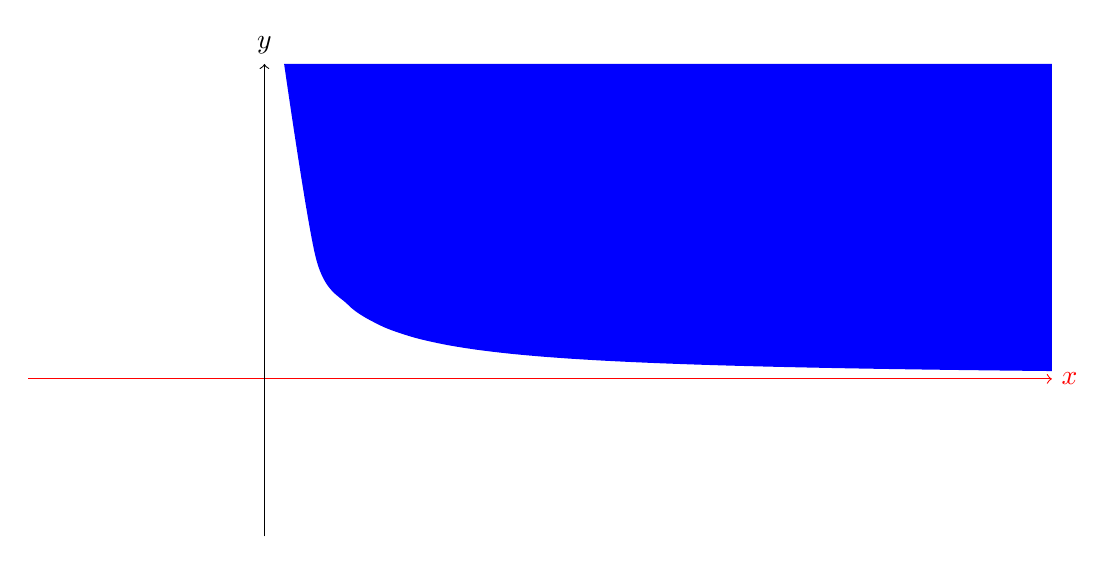
\begin{tikzpicture}
\draw[->, red] (-3,0) -- (10,0) node[right] {$x$};
\draw[->] (0, -2) -- (0,4) node[above] {$y$};
\fill[blue, domain=0.25:10, variable=\x, smooth]
 plot ({\x},{1/\x}) -- (10,1/10)
-- (10,4) -- cycle;
\end{tikzpicture}
\end{proof}
\end{enumerate}
\textbf{6 ** (Recession cones)} Consider a nonempty closed convex 
set $C\subset\E$. We define the \textit{recession cone} of $C$ by 
\begin{equation*}
0^+(C) = \{d\in\E\mid C+\R_+ d\subset C\}.
\end{equation*}
\begin{enumerate}[(a)]
\item Prove $0^+(C)$ is a closed convex cone.
\begin{proof}
If $d^i$ is a sequence in $0^+(C)$ converging to $d$, then 
$C+\R_+d^i\subset C$ for every $i$. Because $C$ is closed, 
$C+\R_+d\subset C$. More explicitly, for any $r\in\R_+$ and $c\in C$, 
$c+rd^i\to c+rd$, and so $c+rd\in C$. \\
To show that $0^+(C)$ is convex, let $x,y\in 0^+(C)$. Then, for any 
$\lambda\in[0,1], r\in\R_+, c\in C$,
\begin{equation*}
\lambda (c+rx) + (1-\lambda)(c+ry) = c+r(\lambda x + (1-\lambda)y).
\end{equation*}
Since $c,r$ were arbitrary, we have $\lambda x+(1-\lambda)y\in 0^+(C)$. 
Since $\lambda,x,y$ were arbitrary, $0^+(C)$ is convex.
\end{proof}
\item Prove $d\in0^+(C)$ iff $x+\R_+d\subset C$ for some point $x$ in 
$C$. Show this equivalence can fail if $C$ is not closed. 
\begin{proof}
The forward implication is obvious. For the backwards implication, 
suppose $x+\R_+d\subset C$ for some $x\in C$. Now let $y\in C, 
r\in\R_+$ be arbitrary. We know that for all $r'\in\R_+$ and $\lambda
\in[0,1]$,
\begin{equation*}
(1-\lambda)y + \lambda(x+r'd) \in C.
\end{equation*}
If we let $\lambda = \frac{r}{r'}$ for $r'\geq r$
 and then take $r'\to\infty$, 
\begin{equation*}
(1-\lambda)y + \lambda(x+r'd) \to y + rd.
\end{equation*}
Because $C$ is closed, $y+rd \in C$. This proves that $C+\R_+d\subset C$.\\
For an example of where this is not true, take\par
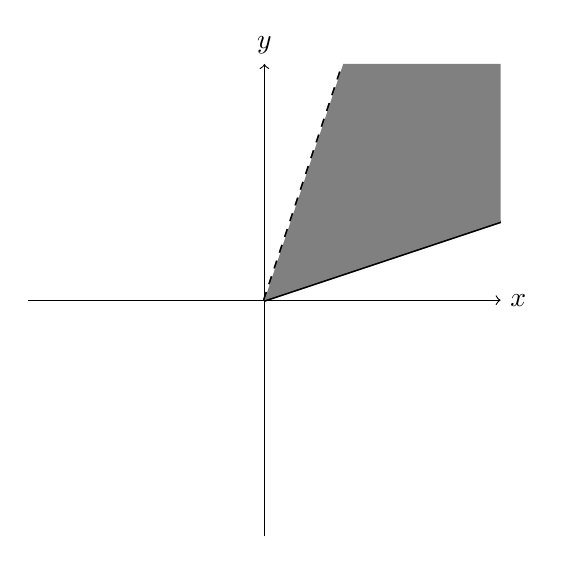
\begin{tikzpicture}
\draw[->] (-3, 0) -- (3,0) node[right] {$x$};
\draw[->] (0, -3) -- (0,3) node[above] {$y$};
\draw[very thick] (0,0) -- (3,1);
\draw[dashed, very thick] (0,0)--(1,3);
\fill[gray] (0,0) -- (3,1) -- (3,3) -- (1,3) -- cycle;
\end{tikzpicture}
\end{proof}
\item Consider a family of closed convex sets $C_{\gamma}(\gamma\in\Gamma)$
with nonempty intersection. Prove $0^+(\bigcap C_\gamma) = \bigcap 
0^+(C_\gamma)$.
\begin{proof}
First, the reverse inclusion. Suppose $d\in \bigcap 0^+(C_\gamma)$.
Then, for every $C_\gamma$, $C_\gamma+\R_+d\subset C_\gamma$. 
Then, if $c\in \bigcap C_\gamma$, we have $c+\R_+d\subset C_\gamma$ 
for every $\gamma\in\Gamma$, i.e. $d \in 0^+(\bigcap C_\gamma)$. \\
For the forward inclusion, suppose $d\in 0^+\left(\bigcap C_\gamma\right)$.
Then for some $x\in\bigcap C_\gamma$, $x+\R_+d\subset \bigcap C_\gamma$.
In other words, for every $C_\gamma$, there is $x\in C_\gamma$ s.t. 
$x+\R_+d \subset C_\gamma$. By the previous part, this implies 
$d\in 0^+(C_\gamma)$. Thus, $d\in\bigcap 0^+(C_\gamma)$.
\end{proof}
\item For a unit vector $u\in\E$, prove $u\in0^+(C)$ iff there is 
a sequence $(x^r)$ in $C$ satisfying $\|x^r\|\to\infty$ and 
$\|x^r\|^{-1}x^r\to u$. Deduce $C$ is unbounded if and only if 
$0^+(C)$ is nontrivial.
\begin{proof}
The proof is similar to that of part (b). Let $y\in C$ and $r\in\R_+$. 
\begin{equation*}
\forall \lambda\in[0,1],\; (1-\lambda)y + \lambda x^i \in C.
\end{equation*}
Let $\lambda = \frac{r}{\|x^i\|}$ for $\|x^i\|\geq r$. Then, the 
above converges to $y+ru$, which is in $C$ because $C$ is closed.
 Since $y,r$ were arbitrary, $u\in 0^+(C)$. \\
Nontriviality of $0^+(C)$ implies there is such a unit vector $u$,
which implies the existence of $\|x^i\|\to\infty$, i.e. unboundedness. 
If $C$ is unbounded, then there is a sequence $x^i$ s.t. $\|x^i\|\to\infty$
where no element is 0.
The sequence $x^i/\|x^i\|$ is contained in the compact $\{x\in\E:\|x\|=1\}$.
Thus, there is a convergent subsequence. The existence of such a 
sequence implies its limit is in $0^+(C)$, i.e. $0^+(C)$ is nontrivial.
\end{proof}
\item If $\Y$ is a Euclidean space, the map $A:\E\to\Y$ is linear, 
and $N(A)\cap0^+(C)$ is a linear subspace, prove $AC$ is closed. 
Show this result can fail without the last assumption. 
\begin{proof}
Let $y^i$ be a sequence in $AC$ converging to $y$. Then, there exists 
a sequence $x^i\in C$ such that $Ax^i\to y$. Each $x^i$ can be 
decomposed into $x^i = u^i+ v^i$ where $u^i\in\range(A^\top)$ and 
$v^i\in N(A)$. Note $Ax^i=Au^i\to y$.
The pseudoinverse $A^+$ satisfies $A^+Ax^i = u^i$ and 
is linear. $A^+$ is continuous because it is linear. Thus, 
\begin{equation*}
u^i = A^+y^i \to A^+y.
\end{equation*}
In other words, the sequence $u^i$ has a limit $u=A^+y$. Next, consider 
the sequence $v^i$. If it is bounded, we can take a convergent 
subsequence to obtain $u^i+v^i\to u+v\in C$, which would imply the 
statement. Otherwise, $v^i$ is unbounded (while $u^i$ is bounded). 
We may assume $v^i/\|v^i\|$ converges to $\hat v$; otherwise we can 
take a convergent subsequence. \\
So, $\|u^i+v^i\|\to\infty$ and $\|u^i+v^i\|^{-1}(u^i+v^i)\to \hat v$.
By part (d), we have $\hat v\in 0^+(C)\cap N(A)$. By assumption, 
$-\hat v\in 0^+(C)\cap N(A)$. This allows us to subtract off the 
component of $\hat v$ in each $v^i$, making $v^i$ perpendicular 
to $\hat v$. We repeat this process until 
the sequence $v^i$ is bounded -- the number of repeats is finite, because 
$\E$ is finite dimensional and we are subtracting off an orthogonal 
component each time. Then, we can take a convergent subsequence of 
$v^i$ to obtain $u^i+v^i\to u+v\in C$ satisfying $A(u+v)=y$. \\
This result may fail without the last assumption. Let $A:\R^2\to\R$
be the projection onto the $y$ coordinate, and let $C$ be the closed 
convex set $\{(x,y): x>0, y\geq 1/x\}$.
 0 is a limit point of $AC$, but it is not contained in $AC$.
\end{proof}
\item Consider another nonempty closed convex set $D\subset\E$ such 
that $0^+(C)\cap0^+(D)$ is a linear subspace. Prove $C-D$ is closed.
\begin{proof}
Let $A:C\times D\to \E$ be the map $A(c,d) = c-d$. Then, $C-D = 
A(C\times D)$. By the above part, if we can show that $N(A)\cap 
0^+(C\times D)$ is a linear subspace, $C-D$ is closed. If 
$u\in 0^+(C)$ and $v\in 0^+(D)$, then for any $(x,y)\in C\times D,
(x,y) + \R_+(u, v) \subset C\times D$. Also, if $(u,v)\in0^+(C\times D)$,
then $x+\R_+u\subset C$ and $y+\R_+v\subset D$. Thus, $0^+(C\times D) 
= 0^+(C)\times 0^+(D).$ Now we note 
\begin{equation*}
N(A)  = \left\{\begin{bmatrix} x \\ x \end{bmatrix}\,\bigg|\, 
x\in C\cap D\right\}.
\end{equation*}
Now let $(x,x)\in N(A)\cap 0^+(C\times D)$. By the above, 
$x\in 0^+(C)$ and $x\in 0^+(D)$. Thus, $x\in 0^+(C)\cap 0^+(D)$. 
Now if $x\in (C\cap D)\cap 0^+(C)\cap 0^+(D)$, then $(x,x)\in 
N(A)\cap0^+(C\times D)$. Also, for any $\alpha\in \R$,
 $\alpha x \in (C\cap D)\cap 0^+(C)\cap 
0^+(D)$, because $x + (\alpha-1)x\in C\cap D$ due to $0^+(C)\cap 
0^+(D)$ being linear, which also gives $\alpha x\in 0^+(C)\cap 0^+(D)$. 
Thus, $(C\cap D)\cap 0^+(C)\cap 0^+(D)$ is linear. Since ``doubling''
each element gives $N(A)\cap 0^+(C\times D)$, $N(A)\cap 0^+(C\times D)$ 
is linear. Thus, $D-C$ is closed.
\end{proof}
\end{enumerate}
\textbf{7. } For any set of vectors $a^1,a^2,\ldots,a^m$ in $\E$, prove
the function $f(x) = \max_i \ip{a^i, x}$ is convex on $\E$.
\begin{proof}
Let $x,y\in\E, \lambda\in[0,1]$. Let $i^*$ be such that 
$f(\lambda x+(1-\lambda)y) = \ip{a^{i^*}, \lambda x + (1-\lambda)y}$. 
We have 
\begin{equation*}
f(\lambda x +(1-\lambda)y) = \lambda\ip{a^{i^*}, x} + (1-\lambda)\ip{
a^{i^*}, y} \leq \lambda f(x) + (1-\lambda)f(y).
\end{equation*}
\end{proof}\noindent
\textbf{8.} Prove Proposition 1.1.3 (Weierstrass). 
\begin{proposition}[Weierstrass]
Let $D\subset\E$ be a nonempty closed set and $f:D\to\R$ continuous 
and with bounded level sets. Then, $f$ has a global minimizer.
\end{proposition}
\begin{proof}
Since $D$ is nonempty, there exists some $\alpha\in\R$ such that 
the level set $\{x\in D : f(x)\leq\alpha\}$ is nonempty. By 
assumption, this level set is bounded. Furthermore, it is closed,
because $f$ is continuous. Thus, it is compact, and $f$ attains a 
minimum over this set. This minimum is also a global minimum of $f$ 
because elements of $D$ outside this set evaluate to greater than $\alpha$.
\end{proof}
\noindent
\textbf{9 (Composing convex functions).} Suppose that the set $C\subset\E$
is convex and that the functions $f_1,f_2,\ldots, f_n:C\to\R$ are 
convex, and define a function $f:C\to\R^n$ with components $f_i$. 
Suppose further that $f(C)$ is convex and that the function $g:
f(C)\to\R$ is convex and \textit{isotone}: any points $y\leq z$ in 
$f(C)$ satisfy $g(y)\leq g(z)$. Prove the composition 
$g\circ f$ is convex.
\begin{proof}
Let $x,y\in C$ and $\lambda\in[0,1]$. Since 
\begin{equation*}
\forall\,i\in[n],\quad
f_i(\lambda x + (1-\lambda)y)\leq \lambda f_i(x)+(1-\lambda)f_i(y),
\end{equation*}
it follows that $f(\lambda x+(1-\lambda)y)\leq \lambda f(x)
+(1-\lambda)f(y)$ elementwise. Therefore,
\begin{equation*}
g(f(\lambda x + (1-\lambda)y)) \leq g(\lambda f(x)+(1-\lambda)f(y))
\leq \lambda g(f(x)) + (1-\lambda)g(f(y)).
\end{equation*}
This proves that $g\circ f$ is convex.
\end{proof}\noindent
\textbf{10 * (Convex growth conditions).}
\begin{enumerate}[(a)]
\item Find a function with bounded level sets which does not satisfy 
the growth condition
\begin{equation*}
\lim_{r\to\infty}\inf\left\{\frac{f(x)}{\|x\|}\bigg|\, 0\neq x\in C,
\,\|x\| = r
\right\} > 0.
\end{equation*}
Take $f(x) = \sqrt{x}$ over the nonnegative reals.
\item Prove any function satisfying the growth condition has bounded 
level sets.
\begin{proof}
Let $r=\liminf f(x)/\|x\|>0$. There exists a constant $\tau$ such that 
if $\|x\|\geq\tau$, then $f(x)/\|x\|\geq r/2$. 
For such $x$, $f(x)\geq r\|x\|/2$. 
Therefore, letting $x\in C$ be arbitrary,
if $f(x)\leq \alpha$, then either $x\leq \tau$ or 
$\|x\|r/2\leq f(x)\leq \alpha$ and $\|x\|\leq 2\alpha/r$. Hence,
$\|x\|\leq \max\{\tau, 2\alpha/r$\}.
\end{proof}
\item Suppose the convex function $f:C\to\R$ has bounded level sets 
but that the growth condition fails. Deduce the existence of a sequence 
$(x^m)$ in $C$ with $f(x^m)\leq \|x^m\|/m \to\infty$. For a fixed 
point $\bar x\in C$, derive a contradiction by considering the 
sequence 
\begin{equation*}
\bar x+(\|x^m\|/m)^{-1}(x^m-\bar x).
\end{equation*}
Hence complete the proof that a convex function 
has bounded level sets iff it satisfies the growth condition.
\begin{proof}
If the growth condition fails, then 
\begin{equation*}
\lim_{r\to\infty} \inf\left\{\frac{f(x)}{\|x\|}\,\bigg|\, 0\neq x \in C,
\, \|x\|=r\right\} \to 0.
\end{equation*}
Then there exists an $r$ such that if $\|x\|\geq r$, then 
$f(x)/\|x\|\leq 1/m$. We can pick such an $x$ that also satisfies 
$\|x\|\geq m^2$. Thus, we deduce the 
existence of the sequence $x^m$ such that $f(x^m) \leq \|x^m\|/m$, and
$\|x^m\|/m \geq m \to\infty$.\\
The sequence $\bar x+(\|x^m\|/m)^{-1}(x^m-\bar x)$ is unbounded because 
\begin{equation*}
\bar x + \left(\frac{\|x^m\|}{m}\right)^{-1}(x^m-\bar x)
= \left(1-\frac{m}{\|x^m\|}\right)\bar x + m \frac{x^m}{\|x^m\|}.
\end{equation*}
Since $m\to\infty$ and the left term goes to $\bar x$, the sequence 
goes to infinite norm. However, on this input, $f$ evaluates to 
something less than 
\begin{equation*}
\left(1-\frac{m}{\|x^m\|}\right)f(\bar x) + (\|x^m\|/m)^{-1}f(x^m)
\leq 2|f(\bar x)| + 1.
\end{equation*}
Thus, the level set corresponding to $2|f(\bar x)|+1$ is unbounded,
giving a contradiction.
\end{proof}
\end{enumerate}
\textbf{11 ** (Accessbility lemma).} Suppose $C$ is a convex set in $\E$.
\begin{enumerate}[(a)]
\item Prove $\cl C\subset C + \epsilon B$ for any real $\epsilon > 0$.
\begin{proof}
For any sequence $x^i\to x$ in $C$, eventually $x^i$ is $\epsilon$ 
close to $x$. Ergo, $x\in C+\epsilon B$.
\end{proof}
\item For sets $D$ and $F$ in $\E$ with $D$ open, prove $D+F$ is open.
\begin{proof}
\begin{equation*}
D+F = \bigcup_{f\in F} D+f.
\end{equation*}
Each $D+f$ is an open set, and the union of open sets is open.
\end{proof}
\item For $x$ in $\inter C$ and $0<\lambda\leq1$, prove $\lambda x + 
(1-\lambda)\cl C\subset C$. Deduce $\lambda\inter C + (1-\lambda)\cl C
\subset \inter C$.
\begin{proof}
Let $x\in\inter C, y\in \cl C$. Since $x\in \inter C$, there is a ball 
of radius some $\epsilon > 0$ centered at $x$ contained in $C$. Let 
$0< \lambda \leq 1$, and denote 
\begin{equation*}
z = \lambda x + (1-\lambda) y.
\end{equation*}
Thus, 
\begin{equation*}
x = \frac{z-(1-\lambda)y}{\lambda}.
\end{equation*}
Take a sequence $y^i$ in $C$ converging to $y$. Let's compute the 
$x'$ for which the convex combination of $x'$ and $y^i$ according to 
$\lambda$ equals $z$. 
\begin{equation}
\label{eq:z}
z = \lambda x' + (1-\lambda)y^i \implies x' = \frac{z-(1-\lambda)y^i}{
\lambda}.
\end{equation}
We have 
\begin{equation*}
\|x-x'\| = \frac{1-\lambda}{\lambda}\|y-y^i\|.
\end{equation*}
Because $y^i\to y$, eventually $\|y-y^i\| \leq \epsilon
\lambda/(1-\lambda)$. This implies $\|x-x'\|\leq \epsilon$. Thus, 
$x'\in C$, since $x+\epsilon B\subset C$. Then \eqref{eq:z} expresses
$z$ as a convex combination of elements in $C$. Thus, $z
= \lambda x + (1-\lambda)y\in C$. Thus, $\lambda x+(1-\lambda)\cl C
\subset C$. \\
$\lambda\inter C + (1-\lambda)\cl C \subset \inter C$ then because 
$\lambda\inter C + (1-\lambda)\cl C$ is open, and a subset of 
$C$.
\end{proof}
\item Deduce $\inter C$ is convex.
\begin{proof}
Since $(1-\lambda)\inter C\subset (1-\lambda)\cl C$, 
\begin{equation*}
\lambda \inter C + (1-\lambda)\inter C \subset \inter C.
\end{equation*}
Thus, $\inter C$ is convex.
\end{proof}
\item Deduce further that if $\inter C$ is nonempty then $\cl\inter C=\cl C$.
Is convexity necessary?
\begin{proof}
Recall by part (c), 
\begin{equation*}
\lambda\inter C+ (1-\lambda)\cl C \subset \inter C.
\end{equation*}
Given $x\in\cl C$, take some $y\in \inter C$ (because $\inter C$ assumed 
nonempty). Then 
\begin{equation*}
\inter C \ni\lambda y + (1-\lambda) x \xrightarrow{\lambda\to\infty}{}
x \in \cl C.
\end{equation*}
We have given a sequence in $\inter C$ converging to $x$. Thus, 
$x\in\cl\inter C$. This proves $\cl C\subset \cl\inter C$. 
w
The other inclusion is trivial.
\end{proof}
\end{enumerate}
\textbf{12 ** (Affine sets)} A set $L$ in $\E$ is \textit{affine} if the 
entire line through any distinct points $x$ and $y$ in $L$ lies in $L$: 
algebraically, $\lambda x+(1-\lambda)y\in L$ for any real $\lambda$. 
The \textit{affine hull} of a set $D$ in $\E$, denoted $\aff D$, is the 
smallest affine set containing $D$. An \textit{affine combination} of 
points $x^1, x^2, \ldots, x^m$ is a point of the form $\sum_{i=1}^m 
\lambda_i x^i$, for reals $\lambda_i$ summing to 1.
\begin{enumerate}[(a)]
\item Prove the intersection of an arbitrary collection of affine sets 
is affine.
\begin{proof}
The proof is similar to the one for convex sets. Let $x,y\in
\bigcap C$, the intersection of a collection of affine sets $\cC$. 
For each $C\in\cC$, $\lambda x+(1-\lambda)y\in C$ for any $\lambda\in\R$.
Thus, $x+(1-\lambda)y\in \bigcap C$. Thus, $\bigcap C$ is affine.
\end{proof}
\item Prove that a set is affine if and only if it is a translate of a 
linear subspace.
\begin{proof}
Suppose $D$ is a translate of a linear subspace, i.e. $D=V+b$ for 
some linear subspace $V$ and $b\in\E$. For any $x+b, y+b\in  D$, we have 
$\alpha x + \beta y \in V$ for all $\alpha,\beta\in\R$. Thus, 
for any $\lambda\in\R$, $\lambda x + (1-\lambda)y\in V$. Thus, 
\begin{equation*}
\lambda(x+b)+(1-\lambda)(y+b) = \lambda x + (1-\lambda)y + b 
\in D.
\end{equation*}
This proves that $D$ is affine. \\
Now suppose that $D$ is affine. If it is empty, we are done. 
Otherwise, take some element $b\in D$, and consider the set 
$V = D-b$. This set is still affine, because if $x, y\in V$, 
then $x+b,y+b\in D$, and so $\lambda x + (1-\lambda)y + b \in D$ 
implying $\lambda x + (1-\lambda)y \in V$ for all $\lambda\in\R$. 
Furthermore, $0\in V$. Thus, 
\begin{equation*}
\forall x \in V, \, \alpha\in \R,\; \alpha x + (1-\alpha)0
= \alpha x \in V.
\end{equation*}
So, for any $x,y\in V$, 
\begin{equation*}
x+y = \frac{1}{2}(2x) + \left(1-\frac{1}{2}\right)2y \in V,
\end{equation*}
because we have written $x+y$ as an affine combination of elements of 
$V$. \\
We have shown $V$ is linear. Then $D=V+b$ is a translate of a linear 
subspace.
\end{proof}
\item Prove $\aff D$ is the set of all affine combinations of elements 
of $D$. 
\begin{proof}
Denote $C = \left\{\sum_{i=1}^m \lambda_i x^i : m\in\N,\,
\sum_{i=1}^m \lambda_i=1,\, x^1,\ldots, x^m\in D\right\}$ as the set 
of affine combinations. \\
First we prove that $C$ is affine. Take $a,b\in C$. Then 
\begin{equation*}
a=\sum_{i=1}^m \lambda_ix^i, \quad b=\sum_{i=1}^{m'} \lambda_i'x'^{i},
\quad \sum_{i=1}^m\lambda_i=\sum_{i=1}^{m'}\lambda_i'=1,\, 
x^i,x'^{i}\in D.
\end{equation*}
For any $\lambda\in\R$,
\begin{equation*}
\lambda a + (1-\lambda)b = \sum_{i=1}^m \lambda\lambda_ix^i
+ \sum_{i=1}^{m'} (1-\lambda)\lambda_i'x'^i \in C,
\end{equation*}
because $\sum_{i=1}^m \lambda\lambda_i + \sum_{i=1}^{m'}(1-\lambda)
\lambda_i' = 1$ and $x^i, x'^i\in D$. Thus, $C$ is affine. \\
Now we prove that an arbitrary affine set $B$ contains all affine 
combinations of its elements. Let $x^1,\ldots,x^m\in B$ and 
$\sum_{i=1}^m \lambda_i=1$. We wish to show that 
$\sum_{i=1}^m \lambda_i x^i \in B$. If $m=2$, this is immediate. 
Now we induct. If $\lambda_1=0$, we may reduce $m$. Otherwise, 
$z=(1-\lambda_1)^{-1}\sum_{i=2}^m \lambda_i x^i\in B$ because it 
is an affine combination of $m-1$ elements. Then 
$\lambda_1 x^1 + (1-\lambda)z \in B$ because $B$ is affine. But 
this is the element we wanted to show was in $B$ to begin with. 
Thus, any affine combination of elements in $B$ is in $B$. \\
Since $C$ is affine and contains $D$, we have $\aff D\subset C$ by 
minimality of $\aff D$. Since $\aff D$ contains $D$ and is affine, 
it contains all affine combinations of elements of $D$. Thus, 
$C\subset \aff D$. Therefore, $\aff D = C$.
\end{proof}
\item Prove $\cl D\subset \aff D$ and deduce $\aff D = \aff(\cl D)$.
\begin{proof}
To show $\cl D\subset \aff D$, it suffices to show that linear subspaces
are closed, because this implies affine sets are closed and then 
the result follows because $\aff D\supset D$. \\
Let $V$ be a linear subspace and suppose $u\notin V$. Then, 
$V$ has an orthonormal basis $v^1,\ldots, v^m$. We have 
\begin{equation*}
u = w+\sum_{i=1}^m c_i v^i, \quad w\neq 0.
\end{equation*}
For any $v\in V$, we then have $\|u-v\|\geq \|w\| > 0$. This eliminates
the possibility of $u$ being a limit point of $V$. Therefore, $V$ is 
closed. \\
$\aff D$ is an affine set containing $\cl D$, so $\aff\cl D\subset 
\aff D$. But clearly $\aff D \subset \aff \cl D$, since 
$D \subset \cl D$. This proves $\aff D = \aff\cl D$.
\end{proof}
\item For any point $x\in D$, prove $\aff D = x+\spn(D-x)$, and deduce 
the linear subspace $\spn(D-x)$ is independent of $x$. 
\begin{proof}
$\aff D \subset x + \spn(D-x)$: Let $\sum_{i=1}^m \lambda_i x^i\in\aff D$.
\begin{equation*}
\sum_{i=1}^m\lambda_i=1,\,\forall\,i\in[m],x^i\in D
\implies \sum_{i=1}^m \lambda_i x^i = x + \sum_{i=1}^m \lambda_i(x^i
- x) \in x+\spn(D-x).
\end{equation*}
$x+\spn(D-x)\subset \aff D$: Let $u-x\in D-x$. We have for all 
$\lambda\in\R$, 
\begin{equation*}
x + \lambda(u-x) = (1-\lambda)x + \lambda u \in \aff D.
\end{equation*}
Then, for any $c_1,\ldots,c_m\in\R$ and $u_1,\ldots, u_m\in D$, 
because $\aff D$ is convex,
\begin{equation*}
x + \sum_{i=1}^m c_i (u_i-x) = \frac{1}{m}\left(\sum_{i=1}^m x+ mc_i(u_i
-x)\right) \in \aff D.
\end{equation*}
This suffices to show that $x+\spn(D-x)\subset\aff D$.
\end{proof}
\end{enumerate}
\textbf{13. ** (The relative interior)} The \textit{relative interior}
of a convex set $C$ in $\E$ is its interior relative to its affine hull, 
$\aff C$, denoted $\ri C$. In other words, a point $x$ lies in $\ri C$ if 
there is a real $\delta > 0$ with $(x+\delta B)\cap \aff C \subset C$.
\begin{enumerate}[(a)]
\item Find convex sets $C_1\subset C_2$ with $\ri C_1\not\subset\ri C_2$.
\text{}\par
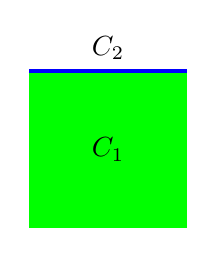
\begin{tikzpicture}
\fill[green] (0,0)--(2,0) --(2,2)--(0,2)--cycle;
\node at (1,1) {$C_1$};
\draw[blue, very thick] (0,2)--(2,2) node[pos=0.5, black, above] {$C_2$};
\end{tikzpicture}
\item Suppose $\dim\E>0,0\in C$ and $\aff C=\E$. Prove $C$ contains 
a basis $\{x^1, x^2, \ldots, x^n\}$ of $\E$. Deduce $\frac{1}{n+1}
\sum_{i=1}^n x^i \in \inter C$. Hence deduce that any nonempty convex 
set in $\E$ has nonempty relative interior.
\begin{proof}
By exercise 12 part (e), $\aff C = \spn(C) = \E$. This implies that 
$C$ contains a basis of $\E$, because we can keep choosing linearly 
independent vectors from $C$ (if we stop early, this implies that 
$\E$ is the span of fewer vectors than the dimension of $\E$, 
a contradiction). \\
\begin{equation*}
\frac{1}{n+1}\sum_{i=1}^n x^i \in \inter C
\end{equation*}
because it is in $C$, and there is a ball around it contained in $C$. 
The latter follows because there exists $\epsilon > 0$ such that 
$\left\|\frac{1}{n+1}\sum_{i=1}^n x^i- x\right\|\leq \epsilon$ 
implies that the unique representation 
\begin{equation*}
x=\sum_{i=1}^n c_i x^i
\end{equation*}
satisfies $\sum_{i=1}^n c_i \leq 1$. This is because there is linear 
mapping $A:\E\to\R^n$ which maps each $x$ to the coefficients of 
$x$ in the basis, and thus $\|A(x_1-x_2)\|\leq \|A\|\|x_1-x_2\|$. 
\\
Then any nonempty convex set in $\E$ has nonempty relative interior, 
because we can shift the set to contain 0, and then consider it 
as a subset of its affine hull, then apply the above argument.
\end{proof}
\item Prove that for $0<\lambda \leq 1$ we have $\lambda\ri C + 
(1-\lambda)\cl C\subset \ri C$, and hence $\ri C$ is convex with $\cl
(\ri C) = \cl C$.
\begin{proof}
Apply parts (c),(d),(e) of 11, setting $\E = \aff C$, so that 
$\inter c = \ri C$.
\end{proof}
\item Prove that for a point $x\in C$, TFAE:
\begin{enumerate}[(i)]
\item $x\in\ri C$. 
\item For any point $y\in C$ there exists a real $\epsilon > 0$ with 
$x+\epsilon(x-y)$ in $C$.
\item $\R_+(C-x)$ is a linear subspace.
\end{enumerate}
\begin{proof}
(i)$\implies$(ii): Because $x\in\ri C$, there exists an $\delta > 0$ 
such that $(x+\delta B)\cap \aff C \subset C$. If $x=y$, the result 
is immediate. Otherwise, $(x-y)/\|x-y\|\subset B$. Therefore, 
\begin{equation*}
x + \frac{\delta}{\|x-y\|}(x-y) \subset (x+\delta B)\cap \aff C
\subset C.
\end{equation*}
Thus, we can take $\epsilon = \delta/\|x-y\|$ to prove the statement.
The inclusion in $\aff C$ is because $x+\epsilon(x-y) = 
(1-(-\epsilon))x + (-\epsilon)y$. \\
(ii)$\implies$(iii): For any $y\in C$, we automatically have 
$y-x\in C-x$. By (ii), we also have $\epsilon(x-y)\in C-x$ for 
some $\epsilon > 0$. This implies that $\R_+(C-x)$ contains 
$\R(y-x)$. Furthermore, $\R_+(C-x)$ is convex, because $\R_+D$ is 
convex for any convex set $D$: if $\alpha x, \beta y\in \R_+D$, 
then for any $\lambda\in[0,1]$,
\begin{equation*}
\lambda \alpha x + (1-\lambda)\beta y = (\lambda\alpha + (1-\lambda)
\beta)\left[\frac{\lambda\alpha x}{\lambda\alpha+(1-\lambda)\beta}
+ \frac{(1-\lambda)\beta y}{\lambda\alpha + (1-\lambda)\beta}\right]
\in \R_+D.
\end{equation*}
This suffices to show that $\R_+(C-x)$ is a linear subspace. \\
(iii)$\implies$(i): 
$\R_+(C-x)$ is a linear subspace implies that for any $y\in C$, 
in addition to $y-x\in C-x$ we have $\epsilon(x-y) \in C-x$. Now for 
any $z\in \aff C = x+\spn{C-x}$ by 12. (e), 
\begin{equation*}
z = x+ \sum_{i=1}^m c_i(x^i-x),\quad \forall i\in[m],\, x^i\in C.
\end{equation*}
For every $x^i$, there exists $\epsilon_i > 0$ such that $\epsilon_i(x-
x^i) \in C-x$. If $c_i\geq 0$, define $z_i=x^i-x$ and $d_i=c_i$, otherwise 
define $z^i = \epsilon_i(x-x^i)$ and $d_i=c_i/\epsilon_i$. Therefore, 
\begin{equation*}
z-x =\left( \sum_{i=1}^m d_i\right)\sum_{i=1}^m
\frac{d_i}{\sum_{j=1}^m d_j} z^i.
\end{equation*}
In other words, $z-x$ is equal to a positive constant times a convex 
combination of elements of $C-x$. But $C-x$ is convex. Therefore, 
it is equal to a positive constant times an element of $C-x$, i.e. 
$z-x\in\R_+(C-x)$. Now let $e^1,\ldots, e^n$ be an orthonormal 
basis for $\aff C-x = \spn{(C-x)}$. By the previous, there exist 
$c_1,\ldots, c_n > 0$ such that $c_ie^i, -c_ie^i\in C-x$ 
for every $i\in[n]$.
This implies that $0\in\ri(C-x)$, i.e. $x\in\ri(C)$.
\end{proof}
\item If $\F$ is another Euclidean space and the map $A:\E\to\F$ is 
linear, prove $\ri AC\supset A\ri C$.
\begin{proof}
Let $y\in A\ri C$. Thus there exists a $x\in\ri C$ such that 
$Ax = y$. We wish to show $y\in \ri AC$. Take $z\in AC$. Then, 
$z=Av$ for some $v\in C$. Then, for some $\epsilon >0$, 
\begin{equation*}
x + \epsilon(x-v)\in C.
\end{equation*}
Then, 
\begin{equation*}
y + \epsilon(y-z) = A(x+\epsilon(x-v)) \in AC.
\end{equation*}
This proves that for any $z\in AC$, there exists $\epsilon > 0$ 
such that $y+\epsilon(y-z) \in AC$. By part (d), this implies that 
$y\in \ri AC$.
\end{proof}
\end{enumerate}
\subfile{1-2/1-2.tex}
\newpage
\section{Chapter 2: Inequality 
constraints}
\subfile{2-1/2-1.tex}
\subfile{2-2/2-2.tex}
\subfile{2-3/2-3.tex}
\section{Chapter 3: Fenchel Duality}
\subfile{3-1/3-1.tex}
\newpage
\subfile{3-2/3-2.tex}
\newpage
\subfile{3-3/3-3.tex}
\newpage
\section{Chapter 4: Convex Analysis}
\subfile{4-1/4-1.tex}
\subfile{4-2/4-2.tex}
\newpage
\subfile{4-3/4-3.tex}
\end{document}
